\part{Theory}
\label{part:theory}
Before implementing our own 3D reconstruction, let's take a  look at some simple theory questions that may arise. The answers to the below questions should be relatively short, consisting of a few lines of math and text (maybe a diagram if it helps your understanding). 

\subparagraph*{Q1.1}\points{5}
Suppose two cameras fixate on a point $\x$ (see \autoref{fig:theory1}) in space such that their principal axes intersect at that point. Show that if the image coordinates are normalized so that the coordinate origin $(0, 0)$ coincides with the principal point, the $\F_{33}$ element of the fundamental
matrix is zero.
\begin{figure}[h]
    \centering
    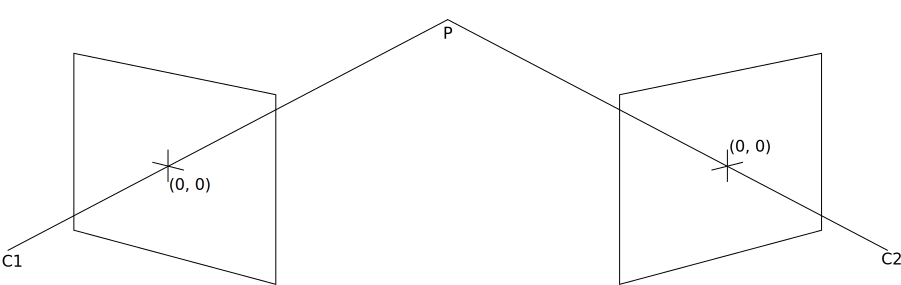
\includegraphics[width=0.75\textwidth]{images/drawing-1.pdf}
    \caption{Figure for Q1.1. $C1$ and $C2$ are the optical centers. The principal axes intersect at point $\w$ ($P$ in the figure).}
    \label{fig:theory1}
\end{figure}

\begin{your_solution}[title=Q1.1,height=6cm,width=\linewidth]
\scriptsize
Under normalized image coordinates, both the principal axes of camera C1 and C2 intersect at a 3D point {\bf w}, plus C1 intercepting at image plane at coordinate $x_1$ = $\begin{bmatrix} 0 \\ 0 \\ 1 \end{bmatrix}$ (in homogeneous coordinate) and C2 intercepting at image plane at coordinate $x_2$ = $\begin{bmatrix} 0 \\ 0 \\ 1 \end{bmatrix}$ (in homogeneous coordinate), then $x_1$ and $x_2$ satisify the following equation: $x_2^T F x_1 = 0$, where F = $\begin{bmatrix}
	F_{11} & F_{12} & F_{13} \\
	F_{21} & F_{22} & F_{23} \\
	F_{31} & F_{32} & F_{33}
\end{bmatrix}$.
When we plug in $x_1$ and $x_2$, it shows that $\begin{bmatrix} 0 & 0 & 1 \end{bmatrix}
\begin{bmatrix}
F_{11} & F_{12} & F_{13} \\
F_{21} & F_{22} & F_{23} \\
F_{31} & F_{32} & F_{33}
\end{bmatrix}
\begin{bmatrix} 0 \\ 0 \\ 1 \end{bmatrix} = 0$, and it results in F33 = 0.
\end{your_solution}

\subparagraph*{Q1.2}\points{5}
Consider the case of two cameras viewing an object such that the second camera differs from the first by a \emph{pure translation} that is parallel to the $x$-axis. Show that the epipolar lines in the two cameras are also parallel. Back up your argument with relevant equations. You may assume both cameras have the same intrinsics.

\begin{your_solution}[title=Q1.2,height=6cm,width=\linewidth]
\scriptsize
Since the two cameras only differ by a pure translation, the rotation matrix R = I (Identity matrix), and the translation matrix $T = [T_x, 0, 0]^T$. Then we have the following equation: $\begin{bmatrix} x_2 & y_2 & 1 \end{bmatrix} K^{-\top} E K^{-1} \begin{bmatrix} x_1 \\ y_1 \\ 1 \end{bmatrix}=0$, where E = $\begin{bmatrix} 0 & 0 & 0 \\ 0 & 0 & -T_x \\ 0 & T_x & 0 \end{bmatrix}$. We can view $K^{-1} \begin{bmatrix} x \\ y \\ 1 \end{bmatrix} = \begin{bmatrix} x_n \\ y_n \\ 1 \end{bmatrix}$ in normalized camer coordinates, then the above equation would be $\begin{bmatrix} x_{n2} & y_{n2} & 1 \end{bmatrix} E \begin{bmatrix} x_{n1} \\ y_{n1} \\ 1 \end{bmatrix}=0$. We now have epipolar line in C2 as $l_2$ = $E \begin{bmatrix} x_{n1} \\ y_{n1} \\ 1 \end{bmatrix} = \begin{bmatrix} 0 \\ -T_x \\ T_xy_{n1} \end{bmatrix}$ $\rightarrow$ $x_{n2}^T\begin{bmatrix} 0 \\ -T_x \\ T_xy_{n1} \end{bmatrix} = -y_{n2}T_x + T_xy_{n1} = 0$ , and epipolar line in C1 as $l_1$ = $E^T \begin{bmatrix} x_{n2} \\ y_{n2} \\ 1 \end{bmatrix} = \begin{bmatrix} 0 \\ T_x \\ -T_xy_{n2} \end{bmatrix}$ $\rightarrow$ $x_{n1}^T\begin{bmatrix} 0 \\ T_x \\ -T_xy_{n2} \end{bmatrix}$ = $y_{n1}T_x - T_xy_{n2} = 0$. We can see that $l_1$ and $l_2$  are both horizontal lines (parallel to the x-axis), and they are parallel to each other.


%We can view $\begin{bmatrix} x_2 & y_2 & 1\end{bmatrix} K^{-\top}$ as camera coordinate of $C2 = [C_{2x}, C_{2y}, C_{2z}]$, and $K^{-1} \begin{bmatrix} x_1 \\ y_1 \\ 1 \end{bmatrix}$ as camera coordinate of $C1 = [C_{1x}, C_{1y}, C_{1z}]^T$. Then, we have the following equation: $\begin{bmatrix} C_{2x} & C_{2y} & C_{2z} \end{bmatrix} E \begin{bmatrix} C_{1x} \\ C_{1y} \\ C_{1z} \end{bmatrix}=0$. The epopolar line in camera C2 = K E  $\begin{bmatrix} C_{1x} \\ C_{1y} \\ C_{1z} \end{bmatrix}$ = $K [0, -T_x C_{1z}, T_xC_{1y}]$

%It turns out to the equation: $\frac{C_{2y}}{C_{2z}} = \frac{C_{1y}}{C_{1z}}$. After multiplying both camera coordinates: $C1 = [C_{1x}, C_{1y}, C_{1z}]^T$ and $C2 = [C_{2x}, C_{2y}, C_{2z}]^T$ by the same intrinsic matrix K and applying the equation: $\frac{C_{2y}}{C_{2z}} = \frac{C_{1y}}{C_{1z}}$, we get image coordinates $y_2$ = $y_1$, showing that the epipolar lines in the two cameras are parallel.
\end{your_solution}

\subparagraph*{Q1.3}\points{5}
Suppose we have an inertial sensor that gives us the accurate positions ($\R_i$ and $\t_i$, the rotation matrix and translation vector) of the robot at time $i$. What will be the effective rotation ($\R_{rel}$) and translation ($\t_{rel}$) between two frames at different time stamps? Suppose the camera intrinsics ($\K$) are known, express the essential matrix ($\E$) and the fundamental matrix ($\F$) in terms of $\K$, $\R_{rel}$ and $\t_{rel}$.

\begin{figure}[h]
    \centering
    \includegraphics[width=0.75\textwidth]{images/F_E}
    \caption{Figure for Q1.3. $C1$ and $C2$ are the optical centers. The rotation and the translation is obtained using inertial sensors. $\R_{rel}$ and $\t_{rel}$ are the relative rotation and translation between two frames.}
    \label{fig:theory3}
\end{figure}

\begin{your_solution}[title=Q1.3,height=17cm,width=\linewidth]
Assume P = $\begin{bmatrix} X_P \\ Y_P \\ Z_P \end{bmatrix}$ is the 3D interception point of camera at time 1 and time 2, that is, camera C1 and C2. Then we have image point in C1 and C2 as $x_1$ and $x_2$ as the following equations:
\begin{align}
	\lambda_1 \begin{bmatrix} x_1 \\ y_1 \\ 1 \end{bmatrix} = K(R_1 \begin{bmatrix} X_P \\ Y_P \\ Z_P \end{bmatrix}) + t_1 \\
	\lambda_2 \begin{bmatrix} x_2 \\ y_2 \\ 1 \end{bmatrix} = K(R_2 \begin{bmatrix} X_P \\ Y_P \\ Z_P \end{bmatrix}) + t_2
\end{align}
The $\lambda_1$ and $\lambda_2$ are the scalar for homogeneous coordinates. When we substitute $\begin{bmatrix} X_P \\ Y_P \\ Z_P \end{bmatrix}$ with $\begin{bmatrix} x_1 \\ y_1 \\ 1 \end{bmatrix}$ in equation (2), then we have the following equation:
\begin{equation}
\begin{split}
	\lambda_2 \begin{bmatrix} x_2 \\ y_2 \\ 1 \end{bmatrix} &= K(R_2 R_1^{-1} (K^{-1} \lambda_1 \begin{bmatrix} x_1 \\ y_1 \\ 1 \end{bmatrix} - t_1) + t_2) \\
	 &= K R_2 R_1^{-1} K^{-1} \lambda_1 \begin{bmatrix} x_1 \\ y_1 \\ 1 \end{bmatrix} - K R_2 R_1^{-1} t_1 + K t_2 \\
	 &= K R_{rel} K^{-1} \lambda_1 \begin{bmatrix} x_1 \\ y_1 \\ 1 \end{bmatrix} + K t_{rel}
\end{split}
\end{equation}
Accordingly, $R_{rel}$ = $R_2 R_1^{-1}$, and $t_{rel} = t_2 - R_2 R_1^{-1} t_1$. Also, the essential matrix E is the cross product of $t_{rel}$ and $R_{rel}$: $E = t_{rel} \times R_{rel}$, and the fundamental matrix F is: $F = K^{-T}(t_{rel} \times R_{rel}) K^{-1}$.


\end{your_solution}